\documentclass[a0paper,portrait]{baposter}
% \documentclass[a0paper,landscape]{baposter}

\input{formatEPISENPoster}

\begin{document}

\begin{poster}{
	% Mettre "true" pour "grid" pour visualiser le placement des boites
	grid=false,
	borderColor=linkEpisenGris,
	headerColorOne=linkEpisenPoster,
	headerColorTwo=linkEpisenPosterLight,
	headerFontColor=black,
	boxColorOne=linkEpisenPosterLight,
	textborder=rectangle,
	bgColorOne=linkEpisenPoster,
	bgColorTwo=linkEpisenMemoireUltraLight,
	headerborder=open,
	boxshade=plain,
	background=shadetb,
	textfont=\large,
	headerfont=\LARGE\sf\bf,
}
{
	% UNUSED
}
{
	% Titre du memoire
	% \smaller \sf \bf \TheManuscritTitle
	\smaller \sf \bf How can we detect cheating effectively without compromising system security through kernel-level access?
}
{
	% Authors
	\smaller \vspace{0.5em} \TheAuthorManuscript\\
	% {\smaller \url{\TheAuthorEmail}}
}
{
	% Logos
	\begin{tabular}{c@{\hskip 2.8cm}c@{\hskip -1.3cm}c}
		\ifthenelse{\equal{\departementEPISEN}{ITS}}
		{
			% ITS
			\begin{minipage}[c][-8ex][b]{0em}
				
\includegraphics[height=2.2cm]{../images/logos/upec-blanc-sans-baseline.png}
			\end{minipage} &
			
\includegraphics[height=3cm]{../images/logos/EPISEN_logo-ITS-blanc-POSTER.png} &
			
\includegraphics[height=2.3cm]{../images/logos/Saint-Gobain-Logo.png}\\
		}
		{
			\ifthenelse{\equal{\departementEPISEN}{SI}}
			{
				% SI
				\begin{minipage}[c][-8ex][b]{0em}
					
\includegraphics[height=2.2cm]{../images/logos/upec-blanc-sans-baseline.png}
				\end{minipage} &
				
\includegraphics[height=3cm]{../images/logos/EPISEN_logo-SI-blanc-POSTER.png} &
				
\includegraphics[height=2cm]{../images/logos/Saint-Gobain-Logo.png}\\
			}
			{
				% ISBS
				\begin{minipage}[c][-8ex][b]{0em}
					
\includegraphics[height=2.2cm]{../images/logos/upec-blanc-sans-baseline.png}
				\end{minipage} &
				
\includegraphics[height=3cm]{../images/logos/EPISEN_logo-ISBS-blanc-POSTER.png} &
				
\includegraphics[height=2.3cm]{../images/logos/Saint-Gobain-Logo.png}\\
			}
		}
	\end{tabular}
}


%%%%%%%%%%%%%%%%%%%%%%%%%%%%%%%%%%%%%%%%%%%%%%%%%%%%%%%%%%%%%%%%
% Ici le debut de vos boites !
%%%%%%%%%%%%%%%%%%%%%%%%%%%%%%%%%%%%%%%%%%%%%%%%%%%%%%%%%%%%%%%%

\begin{posterbox}[name=problematique,span=3,column=0,row=0]{Problem}
    On parle ici du problème en général. On peut rajouter une petite figure. Ici la boîte est sur les 2 colonnes. Elle s'appele ``problematique'' et on peut définir à quelle colonne et ligne elle appartient dans la grille du poster. Ceci est bien sûr qu'un exemple, vous pouvez mettre la première boîte que sur une unique colonne.
    \begin{center}
        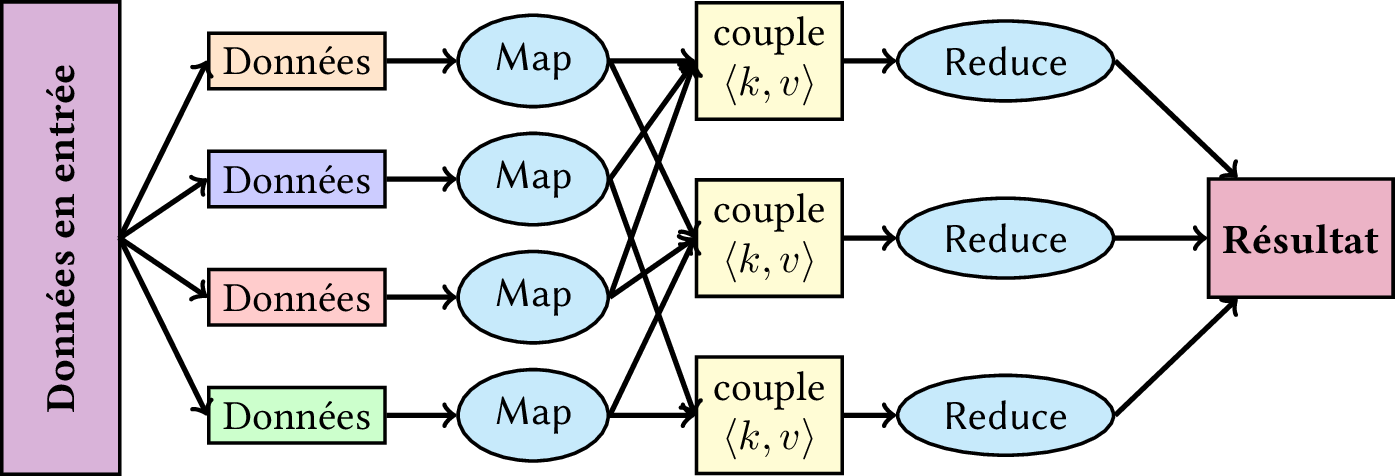
\includegraphics[height=3cm]{../images/Mapreduce.png}
    \end{center}
\end{posterbox}

\begin{posterbox}[name=important,column=1,below=problematique]{Points importants}
    Ici ~; les mêmes points que dans le mémoire car provenant du même fichier~:
    \input{../ShareText/listing1.tex}
\end{posterbox}

\begin{posterbox}[name=formule,span=1,column=2,below=problematique]{Formule importante}
    Ici, LA formule qui est à la base de tout votre mémoire. Exemple~:
    \input{../ShareText/maths1.tex}
    Bien sûr, on peux mettre aussi un algo ou un design de programme ou un protocol ou essai clinique {\it etc.}
\end{posterbox}

\begin{posterbox}[name=tableau,span=2,column=1,below=formule]{Tableau important}
    Ici les données les plus importants de votre travail, identiques à celles de votre mémoire~:
    \begin{center}
        \input{../ShareText/tab1.tex}
    \end{center}
    Sur 2 colonnes car le tableau est un peu gros. Vous trouverez sur le net comment faire
    des tableaux bien plus jolies que cela. Exemples~: \url{https://fr.overleaf.com/learn/latex/Tables}

    Ici, je rajoute du test pour la bibliographie (références)~:
    \begin{itemize}
        \item Un article de revue \cite{ref1}~;
        \item Article de Conférence \cite{ref3}~;
        \item Un livre \cite{ref4}
    \end{itemize}
\end{posterbox}


\begin{posterbox}[name=graph,span=1,column=0,below=problematique]{Un graphe}
    Une autre image~:
    \begin{center}
        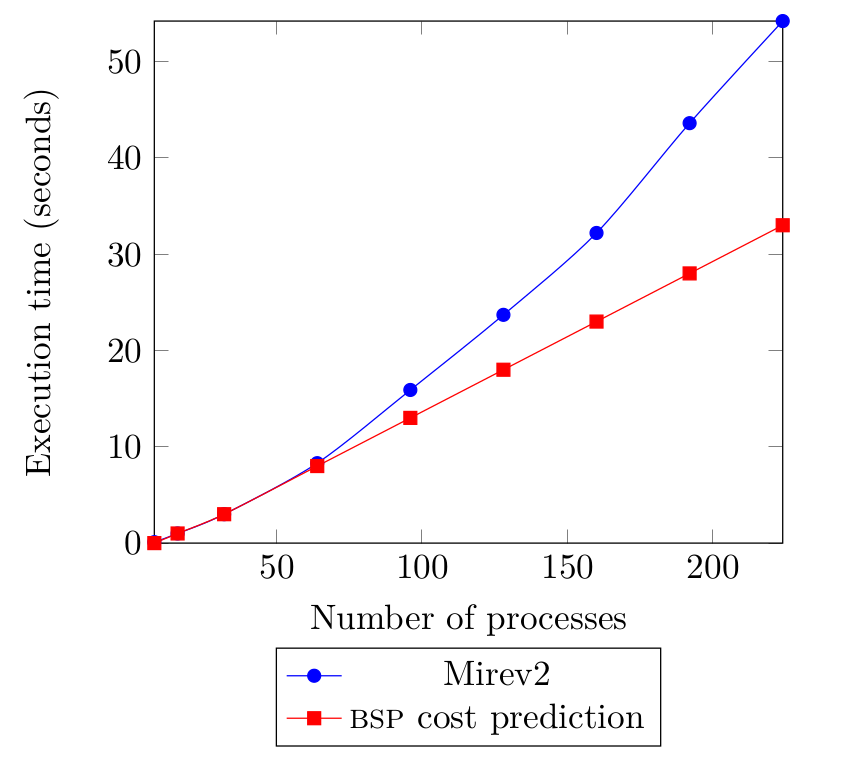
\includegraphics[height=5cm]{../images/reality.png}
    \end{center}
\end{posterbox}

%%%%%%%%%%%%%%%%%%%%%%%%%%%%%%%%%%%%%%%%%%%%%%%%%%%%%%%%%%%%%%%%
%%% Remerciements et bibliographie
%%%%%%%%%%%%%%%%%%%%%%%%%%%%%%%%%%%%%%%%%%%%%%%%%%%%%%%%%%%%%%%%

\ifthenelse{\equal{\TheLanguage}{french}}{
    \begin{posterbox}[name=acknowledgements,column=2,above=bottom]{Remerciements}}
    {\begin{posterbox}[name=acknowledgements,column=2,above=bottom]{Acknowledgements}}
    \smaller
    \vspace{-0.4em}			% Save some space at the beginning
    Ce travail a été effectué avec le soutien de l'EPISEN. Je remercie mon chat, l'EPISEN,
    Gandalf et toute la communauté de l'anneau.
\end{posterbox}

\ifthenelse{\equal{\TheLanguage}{french}}{
    \begin{posterbox}[name=references,column=2,row=0.78]{Références}}
    {\begin{posterbox}[name=references,column=2,row=0.78]{References}}
    \relsize{-5}
    \vspace{-0.4em}
    \setlength{\baselineskip}{0.4em}
    \itemsep=-0.01em
    \renewcommand{\section}[2]{\vskip 0.05em}
    \printbibliography
\end{posterbox}

%%%%%%%%%%%%%%%%%%%%%%%%%%%%%%%%%%%%%%%%%%%%%%%%%%%%%%%%%%%%%%%%
% Ici se termine la déclaration de vos boites !
%%%%%%%%%%%%%%%%%%%%%%%%%%%%%%%%%%%%%%%%%%%%%%%%%%%%%%%%%%%%%%%%

\end{poster}

\end{document}
